\chapter{System Design} \label{chap:System Design}
The first section of this chapter presents the high-level requirements for the system developed in this thesis. The system architecture is explained in detail in the second section. Finally, we explain the design choices and system features with examples.

\section{System Requirements}
Considering the fact that traditional debuggers are not well suited for debugging reactive applications, a new system is developed in this thesis to debug web applications based on JavaScript reactive libraries. We identified the requirements for the system developed in this thesis with regards to the requirements of the software architecture and features available to the end user.\\


%\underline{General Availability}\\
\textbf{General Availability} 
\\
The new system should be easy to install and integrate. In order to reach many developers, the system should be developed as an extension to the widely used Chrome DevTools.\\


\textbf{Debugging without Changing Your Code}
\\
The new system should work without making any change to the application code. Developers should be able to analyze and debug reactive system without modifying the application code.\\


\textbf{Visualization of Application at Macro-Level}
\\
To get the big picture of the application under inspection, the developer should be able to see the dependency graph based on specific time-changing variables (streams/observables). For better understanding of the application, dependencies among different variables should be clearly visible. During the execution of the application, the dependency graph should be automatically updated, so that new variables,
new dependencies, updated values and so forth are immediately visible. Transformation of data streams by different operators should also be visible. Especially, when the chain of operators is being applied to an observable, the transformation should be visible by showing emitted values by each node after applying every single operator in that chain.\\


\textbf{Back-in-Time Debugging}
\\
The developer should be able to have a look at the dependency graph at any arbitrary point in time. Hence, one should be able to visualise the whole history of the dependency graph. Step by step navigation through the time to observe events, such as node creation, value changes, updates of dependencies and the like should be possible. \\


\textbf{Querying the History of the Graph}
\\
Manual step by step navigation is not practical for large programs. Therefore, it should also be possible for the user to jump to a specific point in history with the help of query language.
For example, by defining a query, one should be able to jump to the point in time at which a particular node has been created or evaluated.\\


\textbf{Reactive Breakpoints}
\\
Developers should be able to set breakpoints specific to RP that stop the execution when a significant event occurs. For example, it should be possible to set a breakpoint which hits when a specific node is evaluated, and the evaluation yields a specific value. These breakpoints should be easy to express so that the same query language should be used as mentioned before.\\


\textbf{Extension Helpers}
\\
The developer should have an option to download the dependency graph at any point in time as an image so that it can be shared with other developers. For larger programs, it would be helpful to have a search functionality that finds a node within the dependency graph. For application with long execution cycle, it would be advantageous to have a feature to pause and resume updates to the dependency graph at any point during the execution of an application. \\


\textbf{Library Independence and Extensibility}
\\
The system should not depend on a specific version of reactive libraries implementations, so that if a new version of the reactive library comes then the system should work with little or no modification. It should also be possible to add support for more reactive libraries. The system should be easy to extend, for example, one can easily extend the query language.



\section{System Architecture}

\begin{figure}[!h]
	\centering
	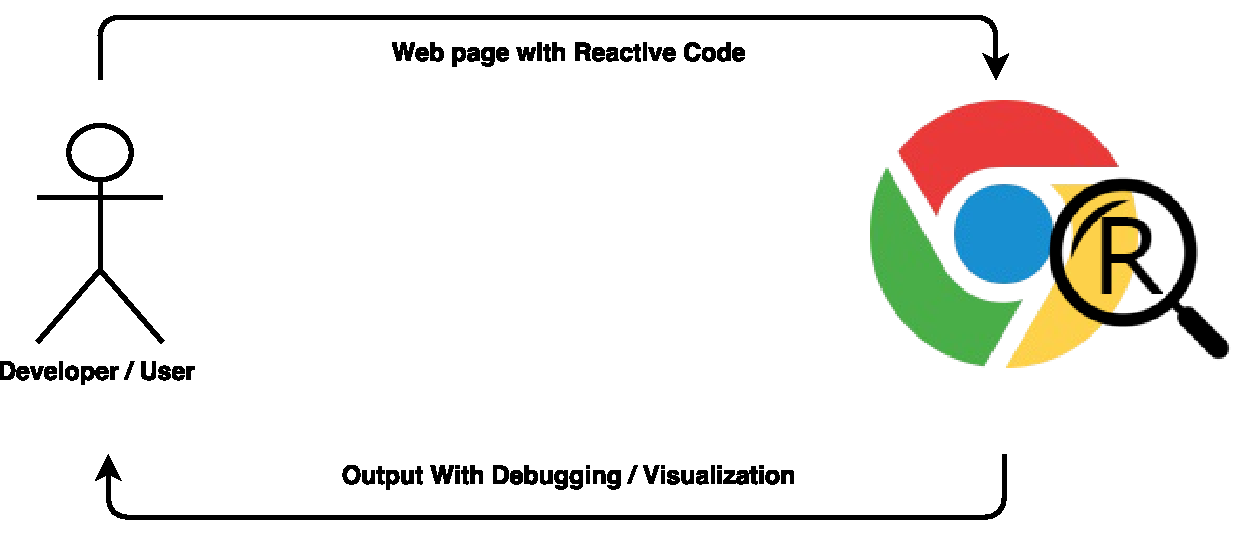
\includegraphics[scale=0.5,trim=0 0 0 0]{gfx/system_design_1.pdf}
	\caption{Simple Use Case Diagram}
	\label{fig:system_design_1-a}
\end{figure}

\begin{figure}[!h]
	\centering
	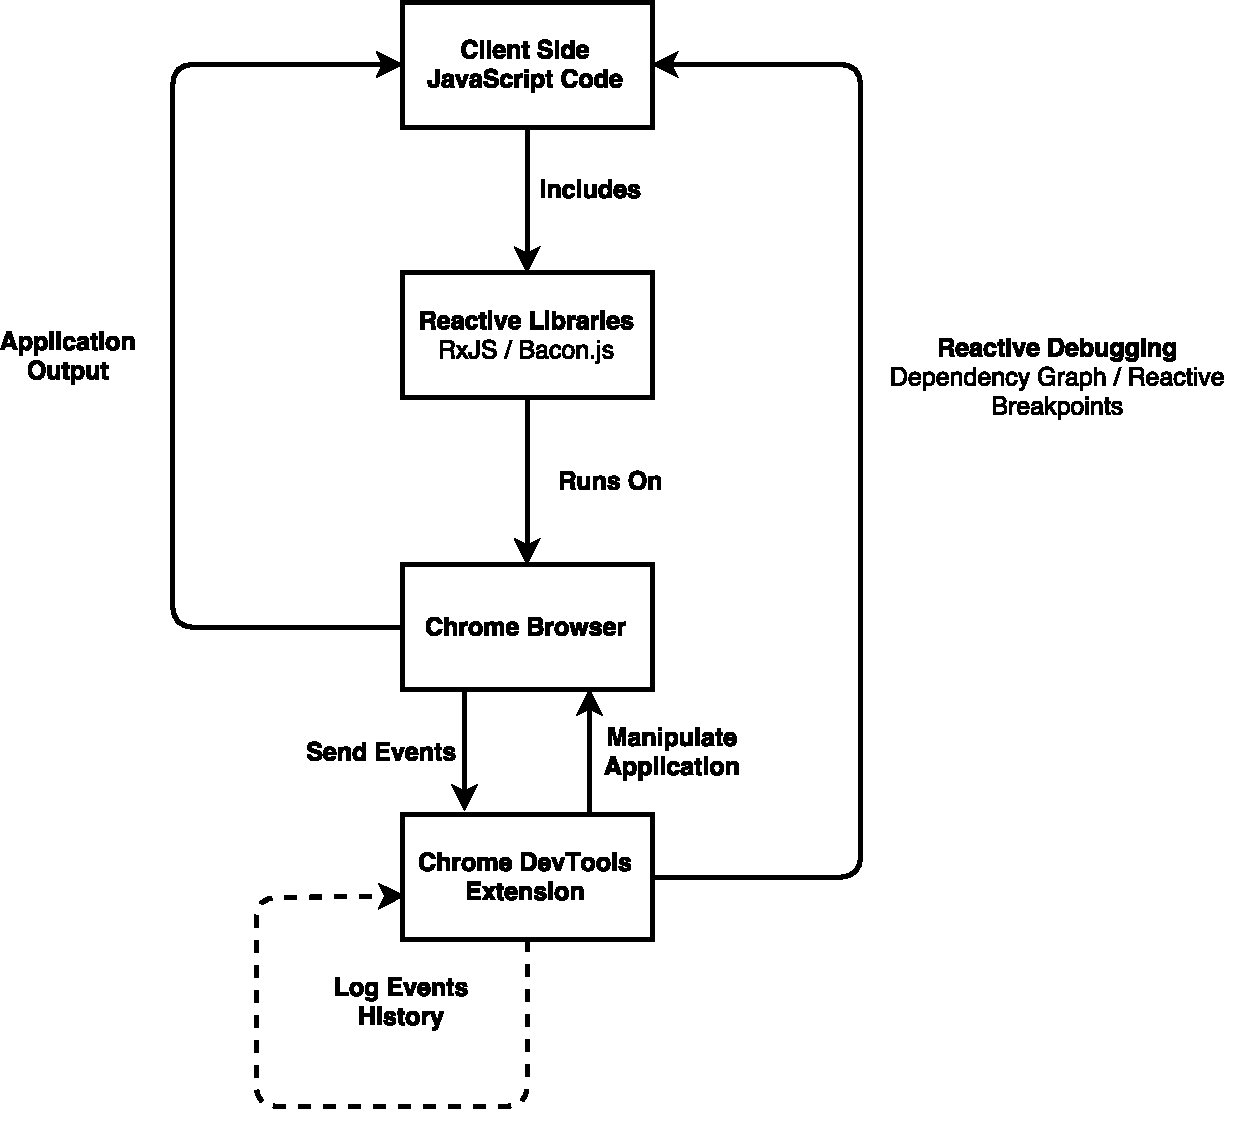
\includegraphics[scale=0.5,trim=0 0 0 0]{gfx/system_design_2.pdf}
	\caption{System Components Overview}
	\label{fig:system_design_2}
\end{figure}

\begin{figure}[!h]
	\centering
	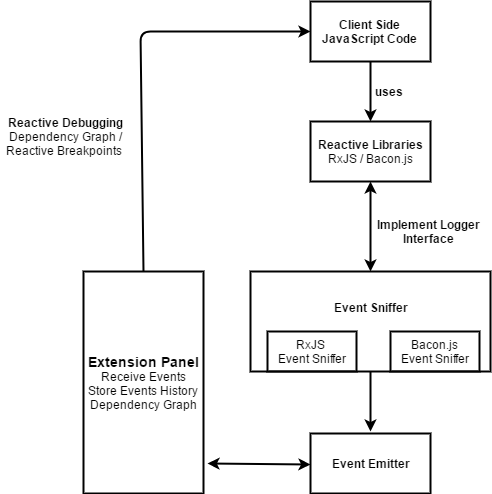
\includegraphics[scale=0.5,trim=0 0 0 0]{gfx/system_design_detail.png}
	\caption{Detailed System Architecture}
	\label{fig:system_design_detail}
\end{figure}

Figure~\ref{fig:system_design_1-a}  shows a simple use case diagram where the developed DevTools extension (CRI) is installed on Google Chrome browser. The user is loading a web application that contains reactive code, in the browser. Chrome browser is returning the output of web application with debugging and visualisation features. 

Figure~\ref{fig:system_design_2} presents the overview of system components and their interaction. CRI manipulates the application code before executing it in the browser. The manipulation makes it possible to sniff all internal events from the reactive library. CRI stores the event history to the browser storage which makes back in time debugging possible. 


Figure~\ref{fig:system_design_detail} depicts the system architecture in detail. The application code is using the reactive library (RxJS / bacon.js). Event Sniffer is a core component of CRI; it contains library specific implementations to sniff all the internal events from the respective library. In this thesis, we have implemented event sniffers for RxJS and bacon.js.
One can easily extend event sniffer to add support for other libraries.
Event Sniffer passes the information to the event emitter, which is further sent to the CRI extension panel. The CRI extension panel receives all event information, it puts this information into defined data structure and saves it to browser storage. The CRI extension panel also creates a dependency graph out of prepared data structure. 


\subsection{Event Sniffing - Options}
To implement the systems architecture mentioned above, the fundamental task at hand was to sniff all internal events from the reactive libraries. Let\textquotesingle s have a look at possible options to implement event sniffer for a particular library.

\subsubsection{Option 1}
The general concept of this option can be visualised in figure~\ref{fig:event_sniffing_1}, where bypass of selected calls to the reactive library is shown. 
We intercept the connection between application code and reactive library and bypass selected calls through injected script. Injected script is JS code that is injected into the web page by CRI. 
This bypass of calls is implemented using AOP technique, which has already been explained in section~\ref{subsec:AOP}.



\begin{figure}[!h]
	\centering
	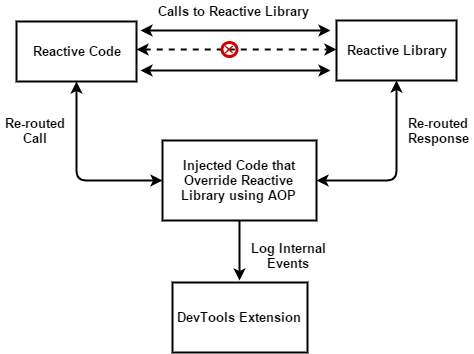
\includegraphics[scale=0.5,trim=0 0 0 0]{gfx/EventSniffing1.png}
	\caption{Event Sniffing - Override Calls To Reactive Library with AOP}
	\label{fig:event_sniffing_1}
\end{figure}

We use this option in event sniffer for RxJS library because RxJS library did not provide any API interface to log all internal activities of the library.  
Although RxJS library provides significantly improved internal architecture from version 5, where they have implemented observables operators in term of \textbf{lift}\footnote{\url{https://github.com/ReactiveX/RxJS/issues/60} , last accessed 23-05-2017}. Lift is a function that takes source observable and an observable factory function and returns a new observable. That means every observable operator of the library calls lift function. We take advantage of this change in the RxJS library, and we just bypass call to lift function of RxJS library using AOP technique. By overriding the only single method of RxJS library, we make it possible to get all observables defined in the application code and then we subscribe to those observables to get their values.



\subsubsection{Option 2}

\begin{figure}[!h]
	\centering
	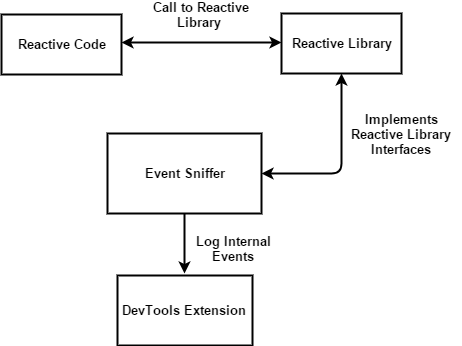
\includegraphics[scale=0.5,trim=0 0 0 0]{gfx/EventSniffing2.png}
	\caption{Event Sniffing - Implementing Interfaces Provided By Reactive Library}
	\label{fig:event_sniffing_2}
\end{figure}

Figure~\ref{fig:event_sniffing_2} depicts the second option to implement event sniffer for the reactive library. For this option, it is necessary that the target library provides some interface to get all internal activities.
Bacon.js provides such interface in term of \textbf{Bacon.spy(f)} \footnote{\url{https://baconjs.github.io/api.html} , last accessed 23-05-2017} method. 
It adds the given function as a spy that will get notified on all new observables. The CRI subscribes to all observables received by the spy interface to sniff all internal events of the library. 


\section{System Features and Design Choices}
\subsection{Dependency Graph Visualization}
As described in chapter~\ref{chap:State of the Art}, reactive systems can be understood and visualised with dependency graphs. A dependency graph consists of nodes and edges where observables are represented by nodes and edges which describe the dependencies among the observables. 

\begin{lstlisting}[language=JavaScript, caption=Bacon.js Example of Up - Down Counter  , label={lst:Bacon_up_down_counter}]
// following observable emit 1 when element with id 'up' is clicked
var upClicks = $('#up').asEventStream('click').map(1);
// following observable emit -1 when element with id 'down' is clicked
var downClicks = $('#down').asEventStream('click').map(-1);
// above two event streams are merged and scaned to get the resultant value
var counter = upClicks.merge(downClicks).scan(0, function(x, y) {
	return x + y;
});
\end{lstlisting}

Consider the following example in listing~\ref{lst:Bacon_up_down_counter} where \textbf{\textit{upClicks}} and \textbf{\textit{downClicks}} are two observables. \textbf{\textit{upClicks}} is a stream of events which emit  \textbf{1} on every click event of DOM element with id is \textbf{\textit{up}}. Similarly \textbf{\textit{downClicks}} observable emits  \textbf{-1} on every click event of DOM element with id is \textbf{\textit{down}}. Line 6 of the example merges both event streams and scan results to the sum of both. The figure~\ref{fig:sys-design_dependency-graph} models our example as a dependency graph and shows the propagation of changes through nodes and edges of the dependency graph. It displays how relevant events affect different parts of the application. Modelling of reactive systems with dependency graphs should be a great help for developers to understand and debug reactive systems.

\begin{figure}[!h]
	\centering
	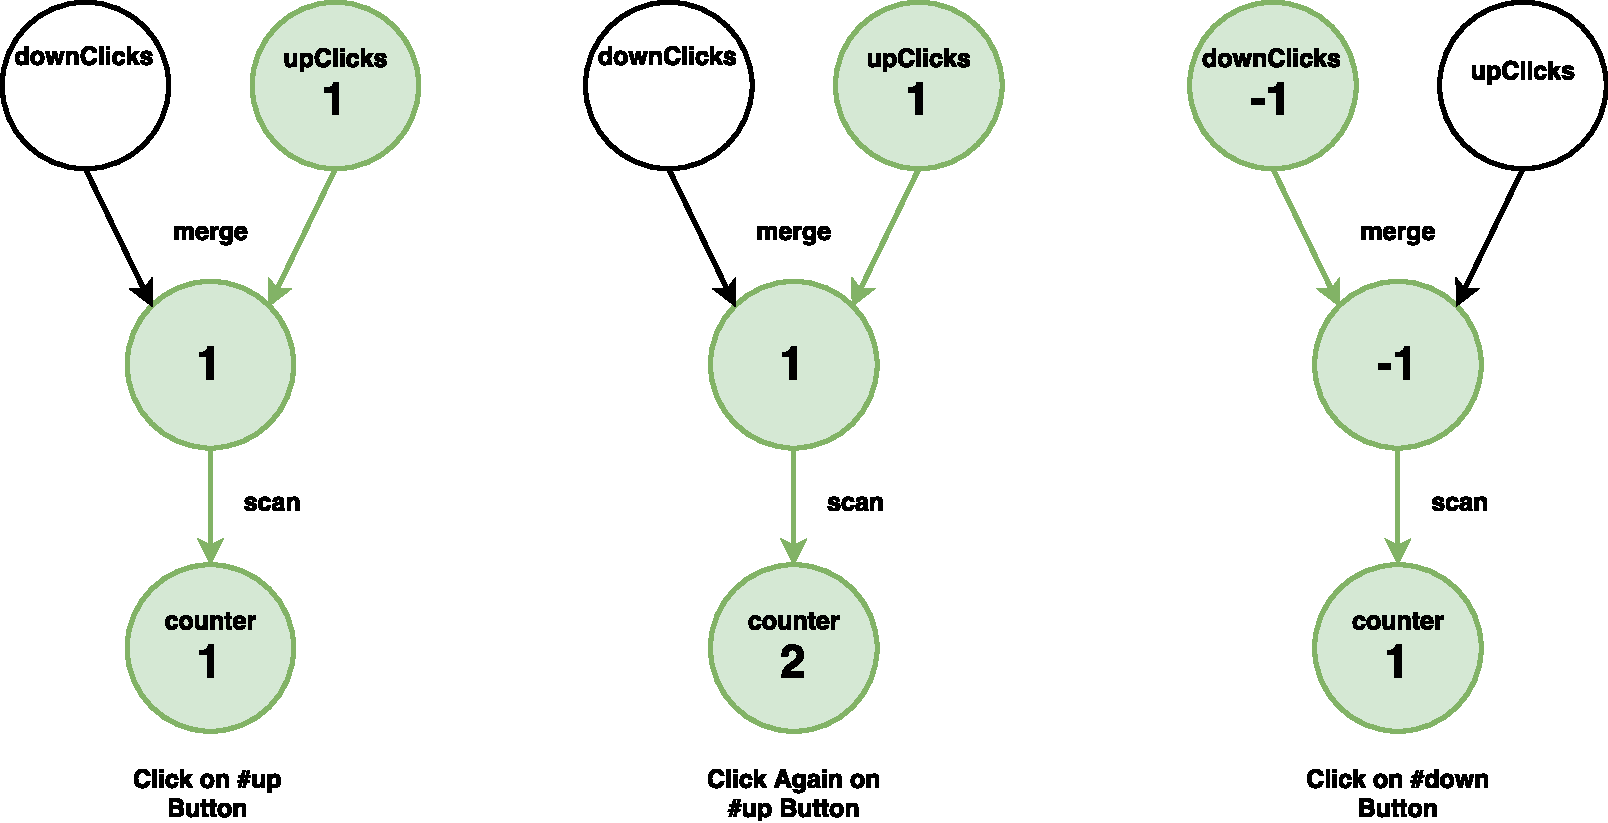
\includegraphics[scale=0.5,trim=0 0 0 0]{gfx/sys-design_dependency-graph.pdf}
	\caption{Propagation of Changes through Dependency Graph}
	\label{fig:sys-design_dependency-graph}
\end{figure}


\subsection{History of Dependency Graph}

During the execution of the reactive application, every change in the dependency graph is recorded as a history of the dependency graph. Hence, the developer has access to the whole history of the
dependency graph. It is possible to see the dependency graph at any point in time. There are three possible ways to navigate through the history. One can use back and forth buttons to navigate step by step through the history of the dependency graph. However step-by-step navigation is not practical with large histories. Developers can use a slider to navigate to arbitrary points in time. A third option to browse through the history is by using the provided query language. Using queries which match certain events, the developer can directly jump to the respective points in time where these events occurred.

\subsection{Reactive Breakpoints}
Native Chrome DevTools support different type of breakpoints to halt the application execution. Most commonly used breakpoints types are, \textbf{line-of-code} and \textbf{conditional line-of-code}
breakpoints \footnote{\url{https://developers.google.com/web/tools/chrome-devtools/javascript/breakpoints} , last accessed 23-05-2017}. These breakpoints are not well suited for RP. Hence, reactive-programming-specific breakpoints should be implemented.
For example, we can set a reactive breakpoint for listing~\ref{lst:Bacon_up_down_counter}, evaluationYielded[nodeIdOfCounter, "2"] query only matches if the \textbf{\textit{counter}} is evaluated to the value \textbf{2}.
This could of course still be done with native DevTools by creating a conditional line-of-code breakpoint at the respective line. But there are also cases which cannot be handled with native DevTools. 
Especially if there is a chain of operators being applied to an observable, then we cannot set breakpoints to intermediate streams with the native debugger.

\subsection{Extension to Chrome DevTools}
The System implemented in this thesis is an extension to Chrome DevTools, which are a set of web authoring and debugging tools built into Google Chrome. Chrome allows the addition of more debugging features to its native debugging tools by creating an extension to DevTools. The developed extension would add a new Panel into the existing Developer Tools of Google Chrome which provides the UI of features discussed so far. The developed extension is so general that the same implementation can also be adopted for others browsers like firefox.


\subsection{Scoping and Snapshot}
The scoping feature aims to decrease performance overhead of the developed extension. As CRI instruments the JavaScript code of the target application with a library called Jalangi. With Scoping feature one can define the target JavaScript file names that should be considered during the instrumentation process. The snapshot feature allows users to download the dependency graph as an image, which they can later share with others. 

\subsection{Reactive Libraries Support}
As mentioned earlier, the system implemented in this thesis supports two reactive libraries, namely RxJS and Bacon.js. In future, one can easily add support for other libraries by implementing event sniffer for that particular library. 

\subsection{Data Storage and Management} \label{subsec:Data_Storage_and_mgmt}
As explained in section~\ref{subsec:Extending_Chrome_DevTools}, different components of Chrome DevTools extension can communicate with each other by message passing. Besides direct communication among extension components, we also need to store data somewhere temporarily. For example, we need temporary storage for the scoping feature, so that we can store the string of file names that a user wants to consider during the instrumentation process. We also need to save reactive breakpoints, so that they can be processed during the execution of target application next time. We use \textbf{chrome.storage}\footnote{\url{https://developer.chrome.com/extensions/storage} , last accessed 23-05-2017} API to store, retrieve and track changes to the user data specific to the features mentioned above. Using this API, we can save objects to local storage of the browser and can access it later from any component of the extension (content script, background, panel).

\subsection{Mapping Stream to JS variable}
During the development of the CRI extension, it was quite challenging to map reactive streams (observables, event stream, property) to the JavaScript variable name defined by the user. For example, if we look into the second line of Listing~\ref{lst:Bacon_up_down_counter}. We can see that there we have an observable that emits 1 when a particular DOM element is clicked. In JavaScript, there is no way to find variable names at runtime. Because the JavaScript interpreter in a browser is implemented as a single thread, only one thing can happen at a time and other actions are queued in execution stack. At runtime, any function can access variables/functions from outside of its own context, but an outside context can not access variables/functions declared inside.
So we can sniff events from our event sniffer without referring those to JavaScript variables names defined by the developer. 

To tackle this issue, we used a third party JavaScript library called Jalangi, which is already introduced in section~\ref{sec:Jalangi}. 
It instruments JavaScript code so that the functionality remains unchanged and the hooks added during the instrumentation process make it possible to monitor every operation (e.g., variable read/write, unary/binary operation, function/method call, etc.) performed by the execution.

\subsection{Chrome Extension Scripts}
Lets the architecture of Chrome DevTools extension from section~\ref{subsec:Extending_Chrome_DevTools} and group the type of JavaScript codes runs in Chrome extension.\\

1) Web Page Scripts: Web Page scripts are the JavaScript code that is part of the webpage, it has full access to the DOM.\\

2) Content Scripts: This runs in a scope between the extension and the web page.  It has partial access to some of the Chrome APIs and full access to the page\textquotesingle s DOM. It executes in a special environment called an isolated world. They do not have access to any JavaScript variables or functions created by the page. It looks to each content script as if there is no other JavaScript executing on the page it is running on. Similarly, Web page scripts cannot call any functions or access any variables defined by content scripts.
An extension can add content script via the manifest file or by using \textbf{chrome.tabs.executeScript} from background script.\\

3) Background Scripts: This behaves as a middle tier in between content and panel script. It can also use to inserting any script as a content script into a page programmatically. Background script has full access to all permitted chrome.* APIs.\\

4) Panel Script: This is responsible for communicating with the background page of extension and the logic of panels and sidebars.\\ 

\subsection{Scripts Injection from Extension}

A Chrome extension can inject JavaScript code into the target application which can be run either in the context of the web page script or in the context of the content script. If the content script\textquotesingle s code should always be injected, then one should register it in the extension manifest using the content\_scripts field\footnote{\url{https://developer.chrome.com/extensions/content_scripts} , last accessed 23-05-2017}.
The content script can also be injected by using \textbf{executeScript} method of tabs API\footnote{\url{https://developer.chrome.com/extensions/tabs} , last accessed 23-05-2017} of Chrome.

\begin{lstlisting}[language=JavaScript, caption=Injecting Script into Web Page Context, label={lst:design_inject_script_to_web_page}]
var scriptElement = document.createElement('script');
scriptElement.src = chrome.extension.getURL('myscript.js');
(document.head || document.documentElement).appendChild(scriptElement);
scriptElement.onload = function() {
scriptElement.parentNode.removeChild(scriptElement);
};
\end{lstlisting}

If we want to inject a script that should be executed in the same context where target web scripts are being run, then we have to inject it by adding new script tag. Listing~\ref{lst:design_inject_script_to_web_page} can be used to inject \textbf{myscript.js} file from the content script into the target web page. We use all of these options to inject script into the web page in our implementations.